\documentclass[11pt, a4paper]{article}
\usepackage[affil-it]{authblk} 
\usepackage{etoolbox}
\usepackage{lmodern}
\usepackage{titlesec}
\usepackage{float}

\makeatletter
\patchcmd{\@maketitle}{\LARGE \@title}{\fontsize{20}{19.2}\selectfont\@title}{}{}
\makeatother

\renewcommand\Authfont{\fontsize{16}{14.4}\selectfont}
\renewcommand\Affilfont{\fontsize{12}{10.8}\itshape}

\title{\textbf{Assignment 2}} 
\author{Pavan R Hebbar - 130010046}
\usepackage{graphicx}
\begin{document}
\maketitle
\newpage
\section{Question 1:}

The following schemes were used to solve the motion of particle in presence of the magnetic field. The value of charge was taken
to be $5$C wih a mass of $10$kg. The value of magnetic field was taken to be $1$T in $\cap{k}$ direction. An initial velocity of
$10^4$ m/s were given to the charge which was initially kept at origin. For the first question we used a time step of 0.01s and 
the final time was taken to be 200s

\subsection{Explicit Euler method}
Following is the plot of the position of the charge over many cycles
\begin{figure}[H]
 \centering
 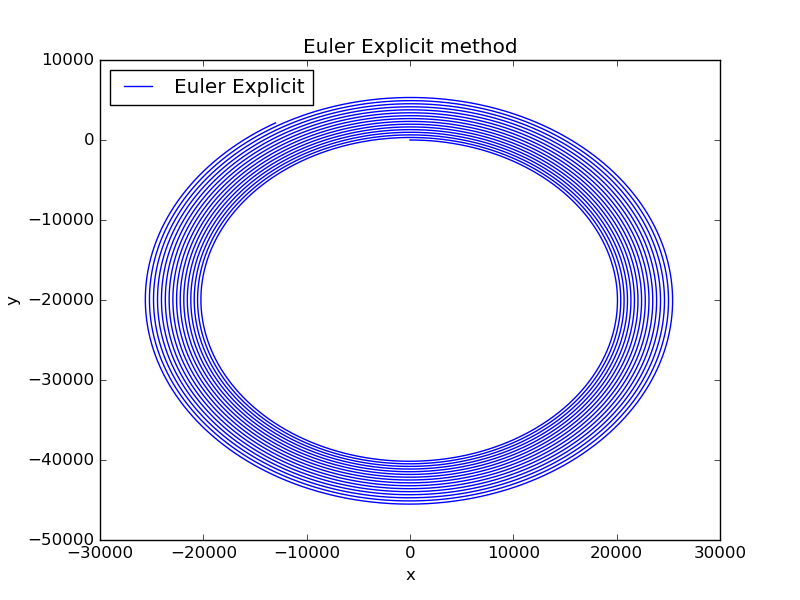
\includegraphics[scale = 0.5]{Euler_exp_1.png}
 \caption{Graph of the position of charged particle over many cycles}
\end{figure}
We see that the particle spirals outwards.
\newpage
The evolution of the energy of the particle is shown in the figure below
\begin{figure}[H]
 \centering
 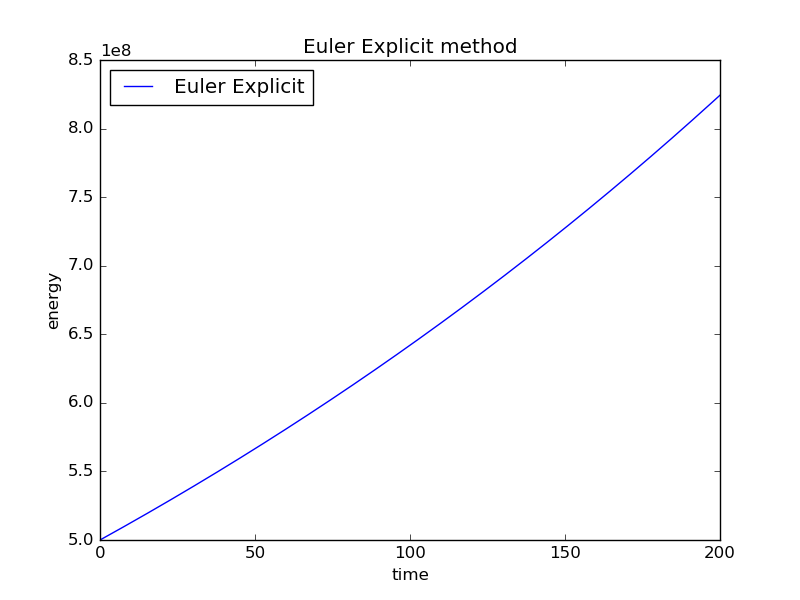
\includegraphics[scale = 0.5]{Euler_exp_en_1.png}
 \caption{Evolution of energy with time}
\end{figure}
Thus the energy of the particle increases quadratically with time

\subsubsection{Position error:}
\begin{equation}
 \Delta (x) = O(\Delta t)
\end{equation}
Following plot shows the variation of error in position with time:
\begin{figure}[H]
 \centering
 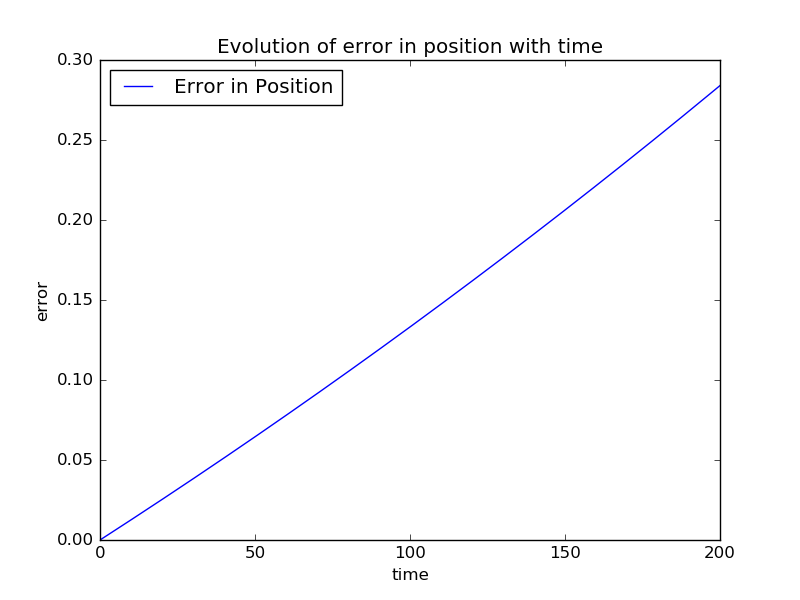
\includegraphics[scale = 0.5]{Eu_err_pos_1.png}
 \caption{Evolution of position error}
\end{figure}


\subsubsection{Dissipation:}
\begin{equation}
 \Delta (E) = O (\delta t)
\end{equation}

\subsection{Semi-implicit Euler:}
Following is the plot of the position of the charge over many cycles
\begin{figure}[H]
 \centering
 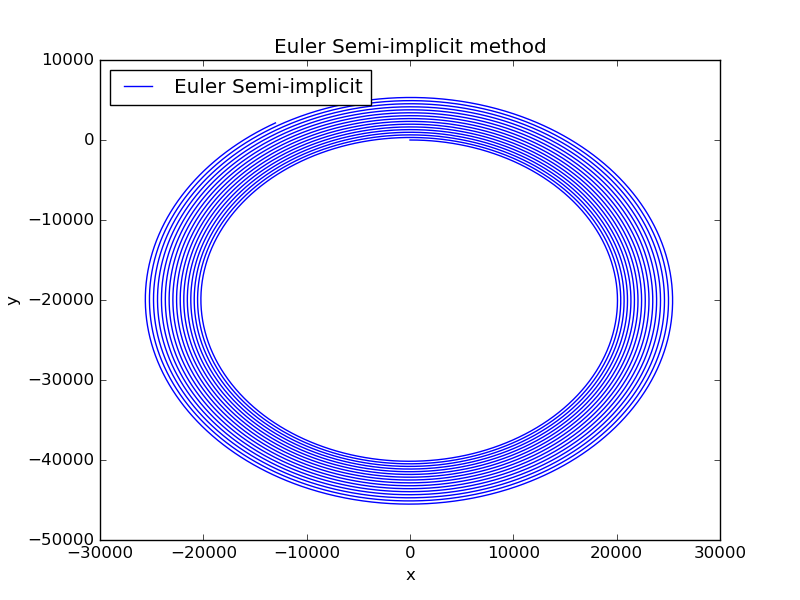
\includegraphics[scale = 0.5]{Euler_sem_1.png}
 \caption{Graph of the position of charged particle over many cycles}
\end{figure}
We see that the particle spirals outwards.
\newpage
The evolution of the energy of the particle is shown in the figure below
\begin{figure}[H]
 \centering
 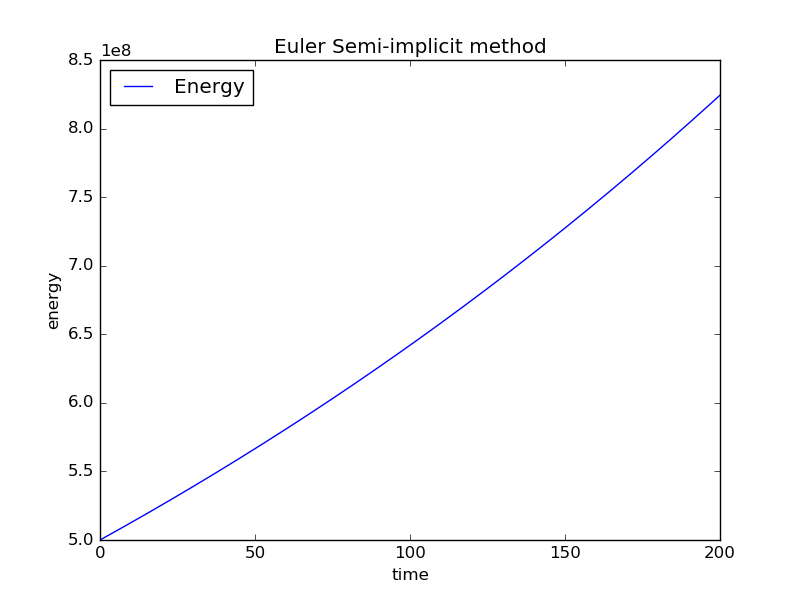
\includegraphics[scale = 0.5]{Euler_sem_en_1.png}
 \caption{Evolution of energy with time}
\end{figure}
Thus the energy of the particle increases quadratically with time

\subsubsection{Position error:}
\begin{equation}
 \Delta (x) = O(\Delta t)
\end{equation}
Following plot shows the variation of error in position with time:
\begin{figure}[H]
 \centering
 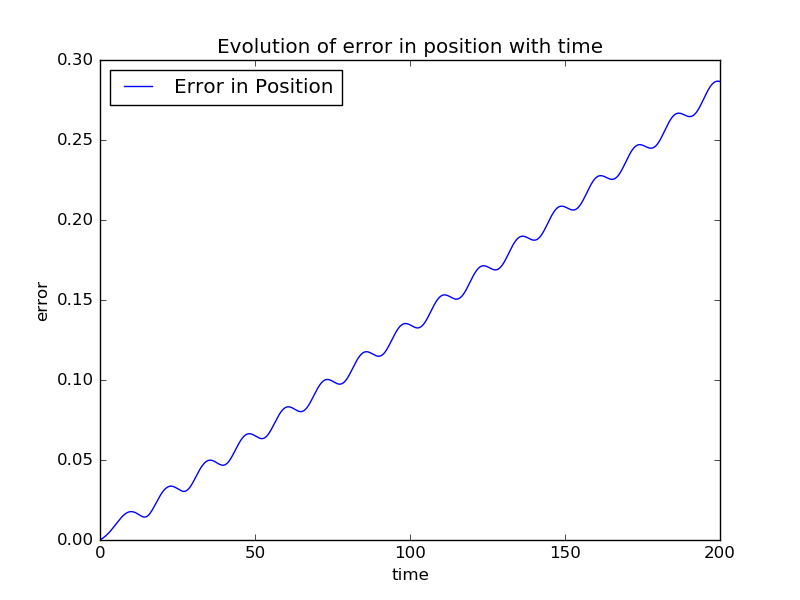
\includegraphics[scale = 0.5]{Sem_err_pos_1.png}
 \caption{Evolution of position error}
\end{figure}


\subsubsection{Dissipation:}
\begin{equation}
 \Delta (E) = O (\delta t)
\end{equation}

\subsection{Runge-Kutta method:}
Following is the plot of the position of the charge over many cycles
\begin{figure}[H]
 \centering
 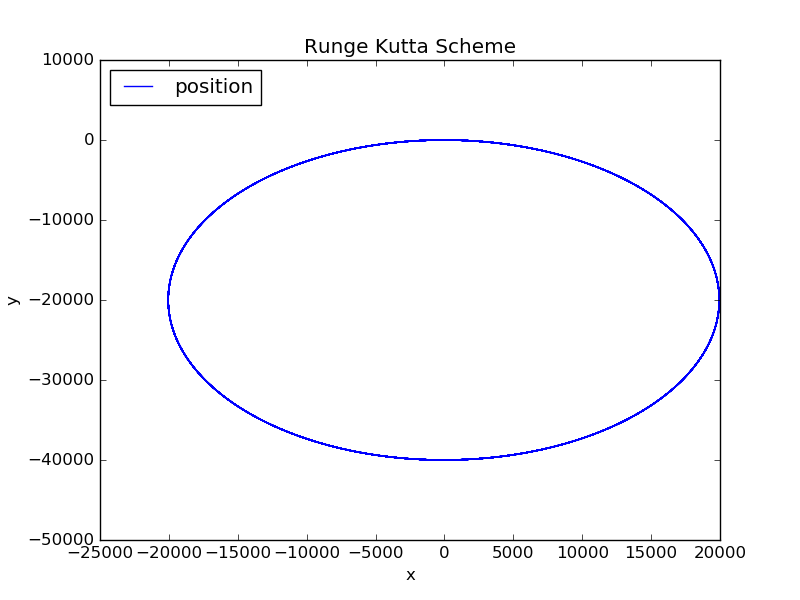
\includegraphics[scale = 0.5]{RK2_pos_1.png}
 \caption{Graph of the position of charged particle over many cycles}
\end{figure}
We see that the particle spirals outwards but very slowly.
\newpage
The evolution of the energy of the particle is shown in the figure below
\begin{figure}[H]
 \centering
 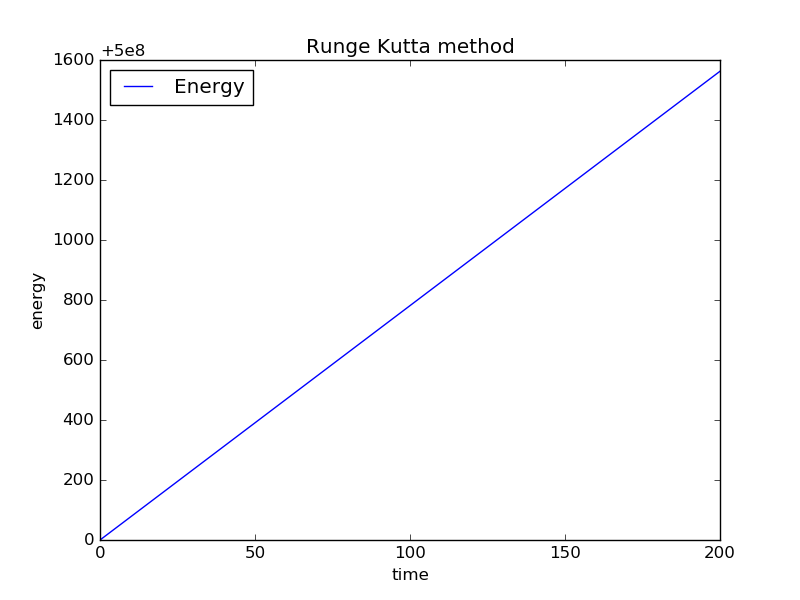
\includegraphics[scale = 0.5]{RK2_en_1.png}
 \caption{Evolution of energy with time}
\end{figure}
Thus the energy of the particle increases quadratically with time

\subsubsection{Position error:}
\begin{equation}
 \Delta (x) = O(\Delta t^{2})
\end{equation}
Following plot shows the variation of error in position with time:
\begin{figure}[H]
 \centering
 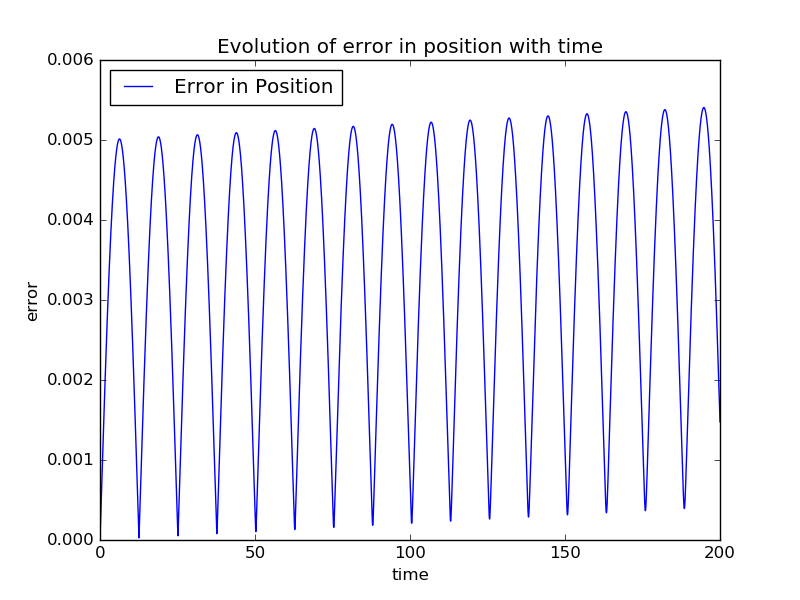
\includegraphics[scale = 0.5]{RK2_err_pos_1.png}
 \caption{Evolution of position error expressed as phase}
\end{figure}


\subsubsection{Dissipation:}
\begin{equation}
 \Delta (E) = O (\delta t)
\end{equation}

\subsection{Boris pusher:}
Following is the plot of the position of the charge over many cycles
\begin{figure}[H]
 \centering
 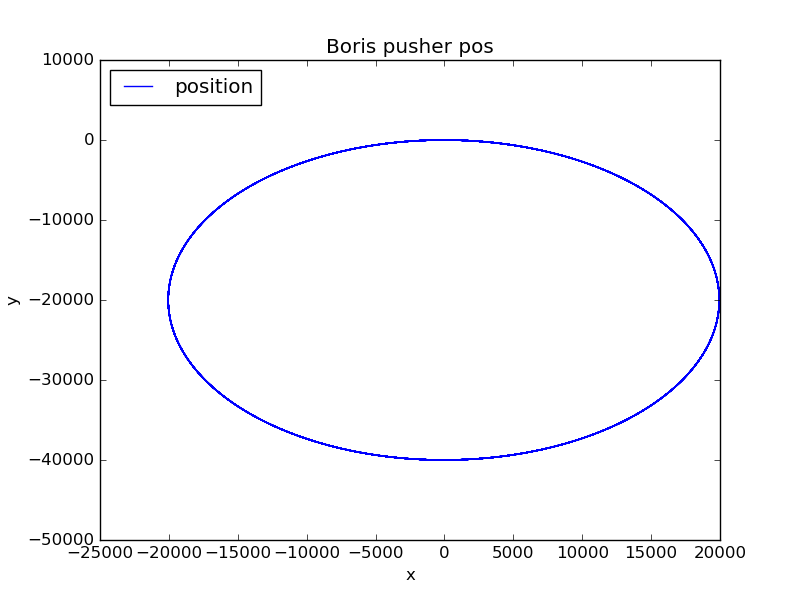
\includegraphics[scale = 0.5]{Boris_pos_1.png}
 \caption{Graph of the position of charged particle over many cycles}
\end{figure}
We see that the particle spirals outwards.
\newpage
The evolution of the energy of the particle is shown in the figure below
\begin{figure}[H]
 \centering
 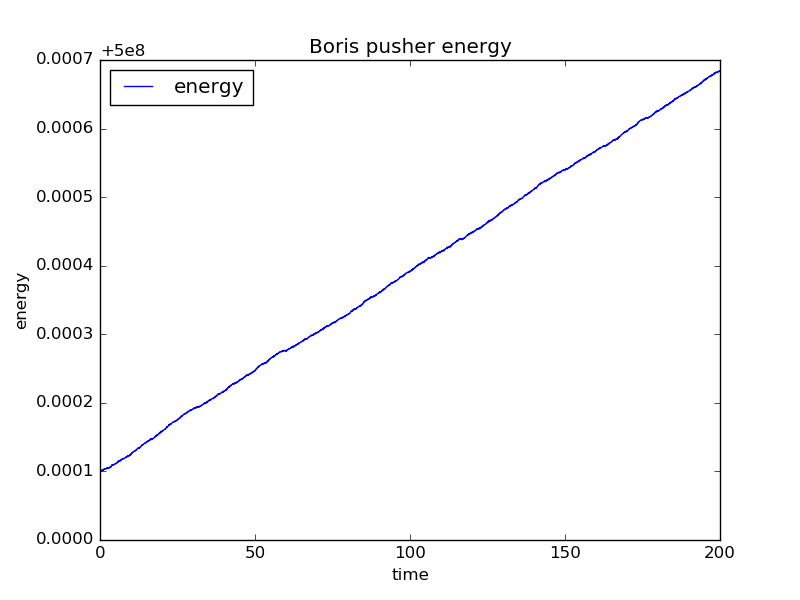
\includegraphics[scale = 0.5]{Boris_energy_1.png}
 \caption{Evolution of energy with time}
\end{figure}
Thus the energy of the particle increases quadratically with time

\subsubsection{Position error:}
\begin{equation}
 \Delta (x) = O(\Delta t)
\end{equation}
Following plot shows the variation of error in position with time:
\begin{figure}[H]
 \centering
 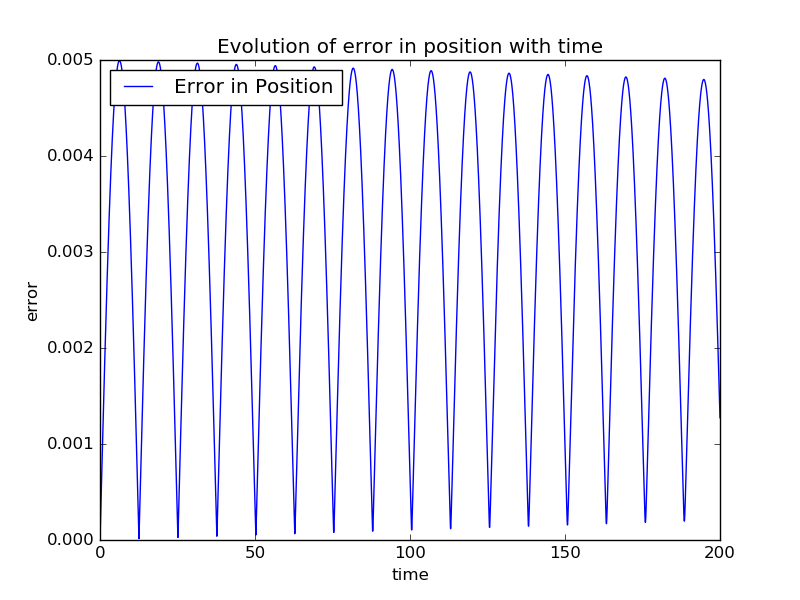
\includegraphics[scale = 0.5]{Bor_err_pos_1.png}
 \caption{Evolution of position error expressed as phase}
\end{figure}


\subsubsection{Dissipation:}
\begin{equation}
 \Delta (E) = O (\delta t)
\end{equation}

\section{Question 2:}
The variation in the position error in various schemes are plotted below
\begin{figure}:
 \centering
 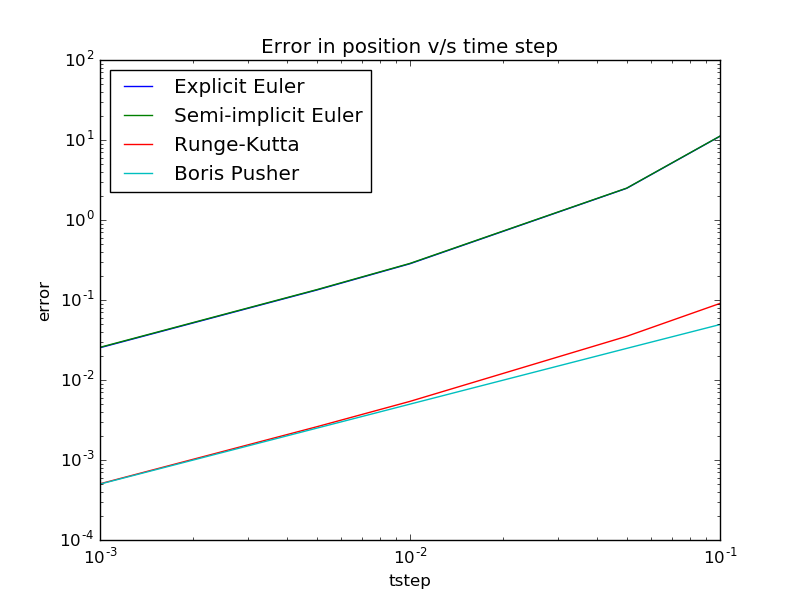
\includegraphics[scale = 0.5]{Pos_err.png}
 \caption{Variation in the position error}
\end{figure}

The variation in energy error in various schemes are plotted below
\begin{figure}:
 \centering
 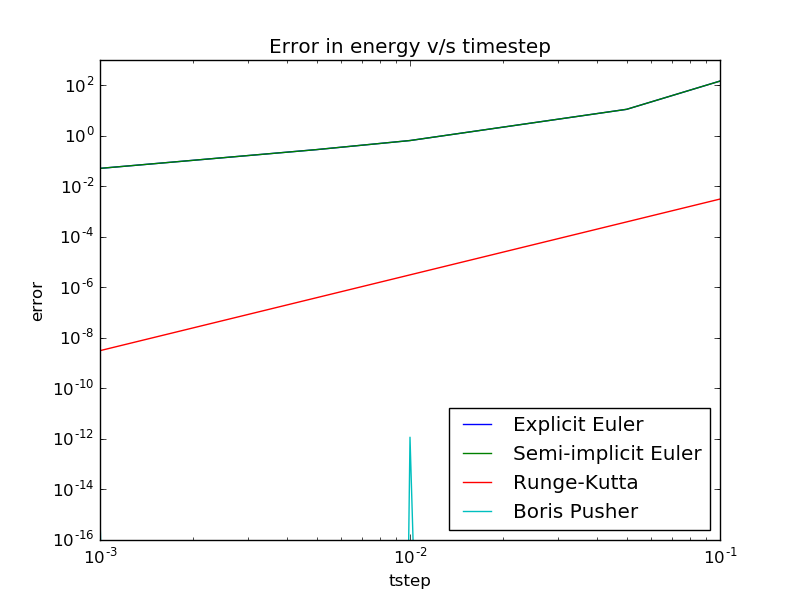
\includegraphics[scale = 0.5]{Energy_err.png}
 \caption{Variation in the position error}
\end{figure}

\section{Question 3:}
The evolution of position of the charge particle is shown below
\begin{figure}[H]
 \centering
 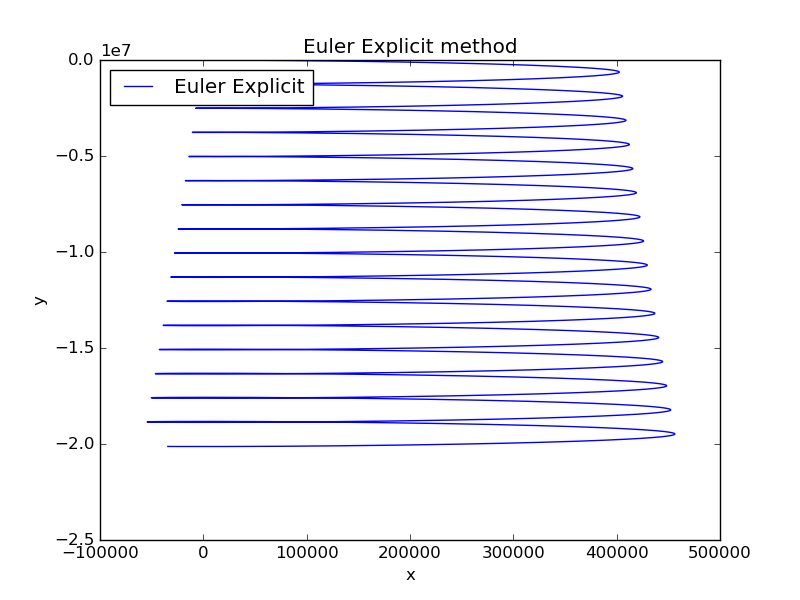
\includegraphics[scale = 0.5]{Euler_exp_2.png}
 \caption{Euler method}
\end{figure}
\begin{figure}[H]
 \centering
 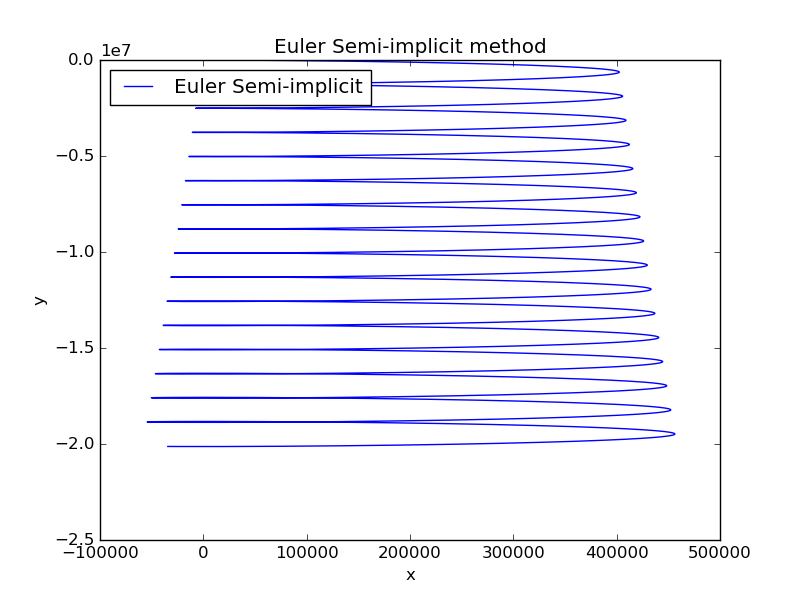
\includegraphics[scale = 0.5]{Euler_sem_2.png}
 \caption{Semi-implicit euler}
\end{figure}
\begin{figure}[H]
 \centering
 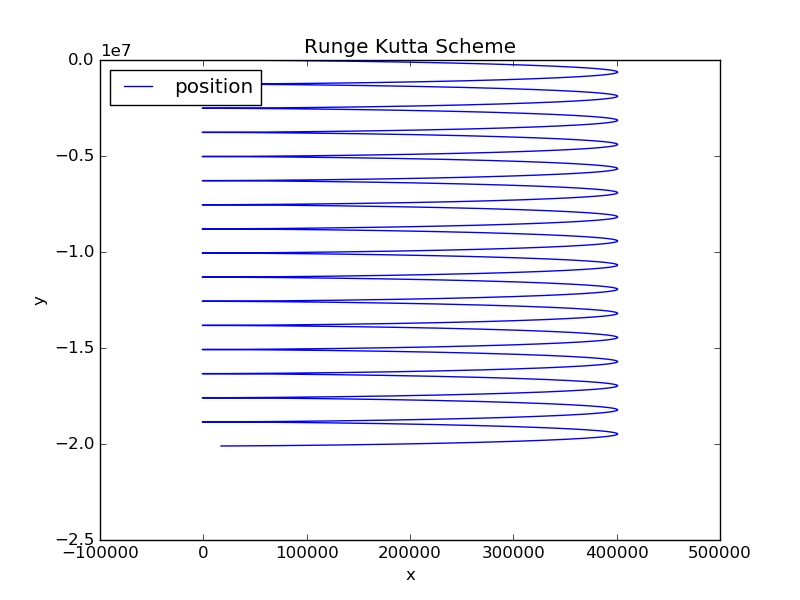
\includegraphics[scale = 0.5]{RK2_pos_2.png}
 \caption{RK2 method}
\end{figure}
\begin{figure}[H]
 \centering
 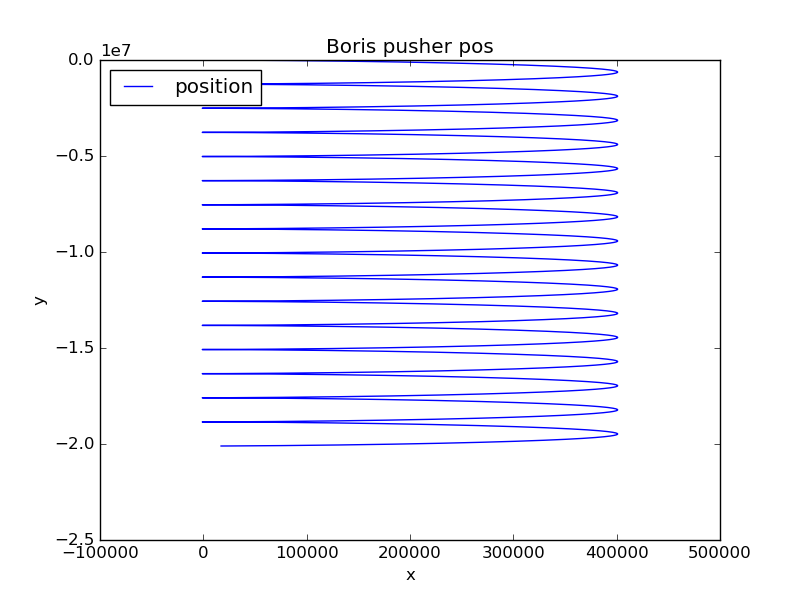
\includegraphics[scale = 0.5]{Boris_pos_2.png}
 \caption{Boris pusher method}
\end{figure}

Observed y positon in Boris pusher method after 200s $=-2.01*10^7$ m/s
Observed x position in Boris pusher method after 200s $=1.71*10^4$ m/s
Since y position due to the gyrating motion will be of the order of $10^4$ and observed is $O(10^7)$, we can say that the 
observed y position is due to the drift velocity
i.e Drift velocity = $-2.01*10^7/200 = -1.005*10^5$ in $\cap{j}$
Calculated drift velocity = $-10^5$
Thus the observed drift velocity is within 1\% of the calculated drift velocity

\section{Question 4:}
The motion of the particle under gradB is shown below
\begin{figure}[H]
 \centering
 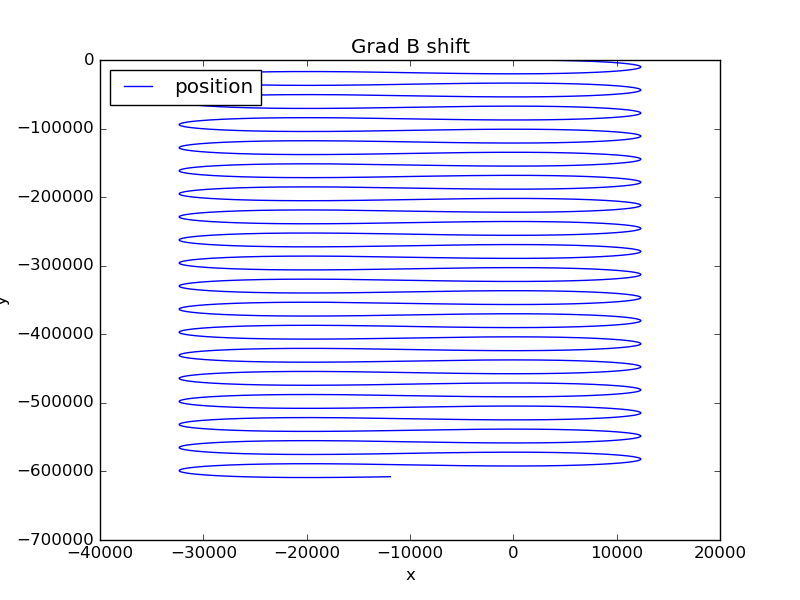
\includegraphics[scale = 0.5]{GradB_boris.png}
 \caption{GradB shift using Boris pusher method}
\end{figure}

\end{document}